% =====================================================================
% Deep Learning Indaba 2026 — Research in Africa Days (RIAD) poster
% Project: mashi-tts-bootstrap
% Size: A0 PORTRAIT (84.1 cm x 118.8 cm), export as PDF
%
% HOW TO USE
%   1. Compile on Overleaf (pdfLaTeX). Upload the whole poster/ folder:
%      this .tex file plus loss_curve.png, mel_comparison.png,
%      qr_repo.png, indaba-logo-white_6-119921388.png,
%      kivuliguaAI_logo.png.
%   2. Numbers marked with a dagger are preliminary estimates calibrated
%      from a one-listener native-speaker assessment; the note under the
%      results table explains this. Replace after the community study.
%   3. The Poster ID box in the title is intentionally blank: write the
%      assigned ID in once the Indaba communicates it.
% =====================================================================
\documentclass[25pt, a0paper, portrait, margin=0mm, innermargin=10mm,
               blockverticalspace=8mm, colspace=12mm, subcolspace=6mm]{tikzposter}

\usepackage[utf8]{inputenc}
\usepackage[T1]{fontenc}
\usepackage{lmodern}
\usepackage{graphicx}
\usepackage{booktabs}
\usepackage{multirow}
\usepackage{amsmath}
\usepackage{xcolor}

% ------- colours ------------------------------------------------------
\definecolor{kivuGreen}{HTML}{1B6B4A}   % main
\definecolor{kivuDark}{HTML}{0E3D2B}
\definecolor{sunGold}{HTML}{E8A13A}     % accent
\definecolor{estRed}{HTML}{B3261E}      % estimated-value marker
\definecolor{paleBg}{HTML}{F4F1E8}

\definecolorstyle{MashiStyle}{}{
  \colorlet{backgroundcolor}{paleBg}
  \colorlet{framecolor}{kivuGreen}
  \colorlet{titlebgcolor}{kivuDark}
  \colorlet{titlefgcolor}{white}
  \colorlet{blocktitlebgcolor}{kivuGreen}
  \colorlet{blocktitlefgcolor}{black}
  \colorlet{blockbodybgcolor}{white}
  \colorlet{blockbodyfgcolor}{black}
  \colorlet{innerblocktitlebgcolor}{sunGold}
  \colorlet{innerblocktitlefgcolor}{black}
  \colorlet{innerblockbodybgcolor}{white}
  \colorlet{notebgcolor}{sunGold!30}
  \colorlet{notefrcolor}{sunGold}
}
\usetheme{Default}
\usecolorstyle{MashiStyle}
\usetitlestyle{Filled}
\useblockstyle{Minimal}

% ------- helper marker ------------------------------------------------
% preliminary calibrated numbers -> red + dagger; see the note under the
% results table. After the community MOS study, redefine \EST to just
% print its argument.
\newcommand{\EST}[1]{\textcolor{estRed}{#1$^{\dagger}$}}

% ------- title banner: logo | title + contributors + ID box | logo ----
% Dark green banner (as in the original design); both logos are white on
% transparent, so they sit directly on the dark background.
\settitle{%
\vspace{4mm}%
\begin{minipage}[c]{0.16\linewidth}
  \centering
  
\includegraphics[width=0.9\linewidth]{indaba-logo-white_6-119921388.png}
\end{minipage}%
\hfill
\begin{minipage}[c]{0.66\linewidth}
  \centering
  {\bfseries\color{white}\fontsize{46}{54}\selectfont
   Bootstrapping TTS for Mashi\par}
  \vspace{4mm}
  {\bfseries\color{white}\fontsize{30}{38}\selectfont
   A First Speech Dataset and XTTS-v2 Fine-Tuning for a\\
   Zero-Resource Bantu Language of DR Congo\par}
  \vspace{6mm}
  {\color{white}\fontsize{26}{32}\selectfont
   Muhigiri Ashuza \quad Marius Nshombo \quad
   Pierre Matabaro \quad David Namulabarha\par}
  \vspace{5mm}
  {\color{white}\large\setlength{\fboxsep}{4mm}\setlength{\fboxrule}{0.6mm}%
   \fbox{\textbf{Poster ID:}\hspace{35mm}\rule{0pt}{7mm}}\par}
\end{minipage}%
\hfill
\begin{minipage}[c]{0.16\linewidth}
  \centering
  
\includegraphics[width=0.95\linewidth]{kivuliguaAI_logo.png}
\end{minipage}%
\vspace{4mm}%
}

\begin{document}
\maketitle[width=0.97\linewidth]

\begin{columns}

% =====================================================================
\column{0.5}
% =====================================================================

\block{1. Motivation: 3 million speakers, zero tools}{
\textbf{Mashi} (Shi, ISO 639-3: \texttt{shi}) is a Bantu language spoken by
$\sim$3 million people in South Kivu, eastern DRC (Ngweshe, Nyangezi,
Bunyakiri, Muganzo). Before this project it had \textbf{no} TTS, ASR, NLP
dataset, or language model of any kind. Related languages (Kinyarwanda,
Kirundi) are themselves low-resource and absent from mainstream TTS models.

\vspace{3mm}
\innerblock{Research question}{Can fine-tuning a multilingual TTS model
(Coqui XTTS~v2) on \textbf{$\sim$1 hour} of curated Mashi audio produce
intelligible Mashi speech?}

\vspace{3mm}
Speech-first access matters: many speakers read French or Swahili rather
than written Mashi, so \emph{voice} interfaces are the natural entry
point for local-language technology.
}

\block{2. Contribution 1: the first Mashi speech dataset}{
\textbf{723 clips / 67.4 minutes} of segmented, transcribed, TTS-ready
audio (22\,050 Hz mono WAV, 2.0--11.3 s, cut only at natural pauses),
built from $\sim$10 h of raw audio across \textbf{3 speakers} and
\textbf{5 domains}:

\vspace{3mm}
\begin{tabular}{@{}llrr@{}}
\toprule
\textbf{Speaker} & \textbf{Domain} & \textbf{Clips} & \textbf{Min} \\
\midrule
bib (M, $\sim$35) & Bible: Genesis ch.\,1--4    & 183 & 24.2 \\
dav (M, 51)       & Short stories / folk tales  & 109 & 12.5 \\
dav               & Numbers (esabu)             &  39 &  3.5 \\
dav               & Family vocabulary           &  25 &  3.0 \\
dav               & Calendar (nsaha)            &  31 &  3.3 \\
mrl (F, $\sim$28) & Clock-time expressions      & 336 & 20.9 \\
\midrule
\textbf{Total}    &                             & \textbf{723} & \textbf{67.4} \\
\bottomrule
\end{tabular}

\vspace{3mm}
{\small Split: \textbf{687 train / 36 eval}, stratified per speaker and
domain (seed 42). Sources: Padri P.~Matabaro's Mashi Bible audio
(bible.com), original texts read by D.~Namulabarha, and murhula.com
talking-clock components (permission: M.~Nshombo). \emph{Disclosure:} the
clock-time domain recombines 95 unique component recordings, the same way
the source site plays them.}
}

\block{3. Contribution 2: a low-cost curation pipeline}{
A reproducible recipe for collectors with no lab and no GPU:

\vspace{2mm}
\begin{itemize}
  \item \textbf{Silence-based segmentation at natural pauses.} Narrative
        audio is split only at detected silences, so no word is ever cut.
        Vocabulary recordings (one item per pause) segment themselves.
  \item \textbf{Component-based synthesis of clock-time clips.} Hour and
        minute announcements from a public talking clock are assembled
        into full time expressions: 10 min of source audio becomes 336
        aligned clips.
  \item \textbf{Text normalization:} casing and apostrophe policy for a
        Latin-based orthography with diacritics (\^{e}, \^{a}, \^{i}, \^{u}).
  \item \textbf{Everything transcribed and verified by a native/heritage
        speaker}, with per-clip provenance and permissions in a data card.
\end{itemize}

\vspace{2mm}
\coloredbox{Total cash cost of the dataset: \textbf{$\approx$\,\$0}
(phone recordings + public sources + consent), plus curation time.}
}

\block{4. Model \& training setup}{
\textbf{Base:} Coqui \textbf{XTTS v2} (multilingual, voice-cloning GPT +
HiFi-GAN decoder). None of its 17 languages is Bantu, so we use
\textbf{Spanish as a phonetic proxy}: it shares Mashi's five pure vowels
/a e i o u/ and open CV syllable structure, and its text frontend expands
clock digits (``9:05'') deterministically at train \emph{and} inference time.

\vspace{2mm}
\begin{itemize}
  \item Fine-tune the GPT component on 687 clips; eval on 36 held-out clips.
  \item \textbf{10 epochs}, batch 8 $\times$ grad-accum 2 (effective 16),
        max clip 11.6 s.
  \item Hardware: one \textbf{A100} on Modal; total fine-tune wall clock
        under 2 h, reproducible for $\approx$\,\$5--10 of cloud credit.
  \item Voice conditioning at inference from one reference WAV per speaker.
\end{itemize}
}

\block{5. How our numbers compare to published systems}{
{\footnotesize
\begin{tabular}{@{}llll@{}}
\toprule
\textbf{System} & \textbf{Data} & \textbf{Setting} & \textbf{Result} \\
\midrule
BibleTTS (VITS) & 33--87 h        & 6 African languages     & MOS 2.8--4.3 in-dom., 2.3--3.9 out-dom. \\
BnTTS (XTTS)    & 3\,850 h + 20 min/spk & Bangla few-shot adaptation & SMOS 4.62, CER 0.034 \\
Align2Speak     & 0.5--5 h        & unseen lang., fine-tune + GRPO & CER 33\% $\rightarrow$ 3.9\% (Portuguese) \\
\textbf{Ours}   & \textbf{1.1 h}  & \textbf{unseen Bantu, Spanish proxy} & \EST{MOS 2.5--3.5} \\
\bottomrule
\end{tabular}}
\\[2mm]
{\small With 30$\times$ less data than BibleTTS's smallest language and no
large-scale target-language pre-training (unlike BnTTS), we expected
results below those systems, and the preliminary evaluation (Section 6)
confirms this. The claim under test is \textbf{intelligibility}, not
studio quality.}
}

% =====================================================================
\column{0.5}
% =====================================================================

\block{6. Results \textmd{\small ($^{\dagger}$ = preliminary calibrated
estimate; see the note under the table)}}{

\innerblock{Training}{
\begin{center}
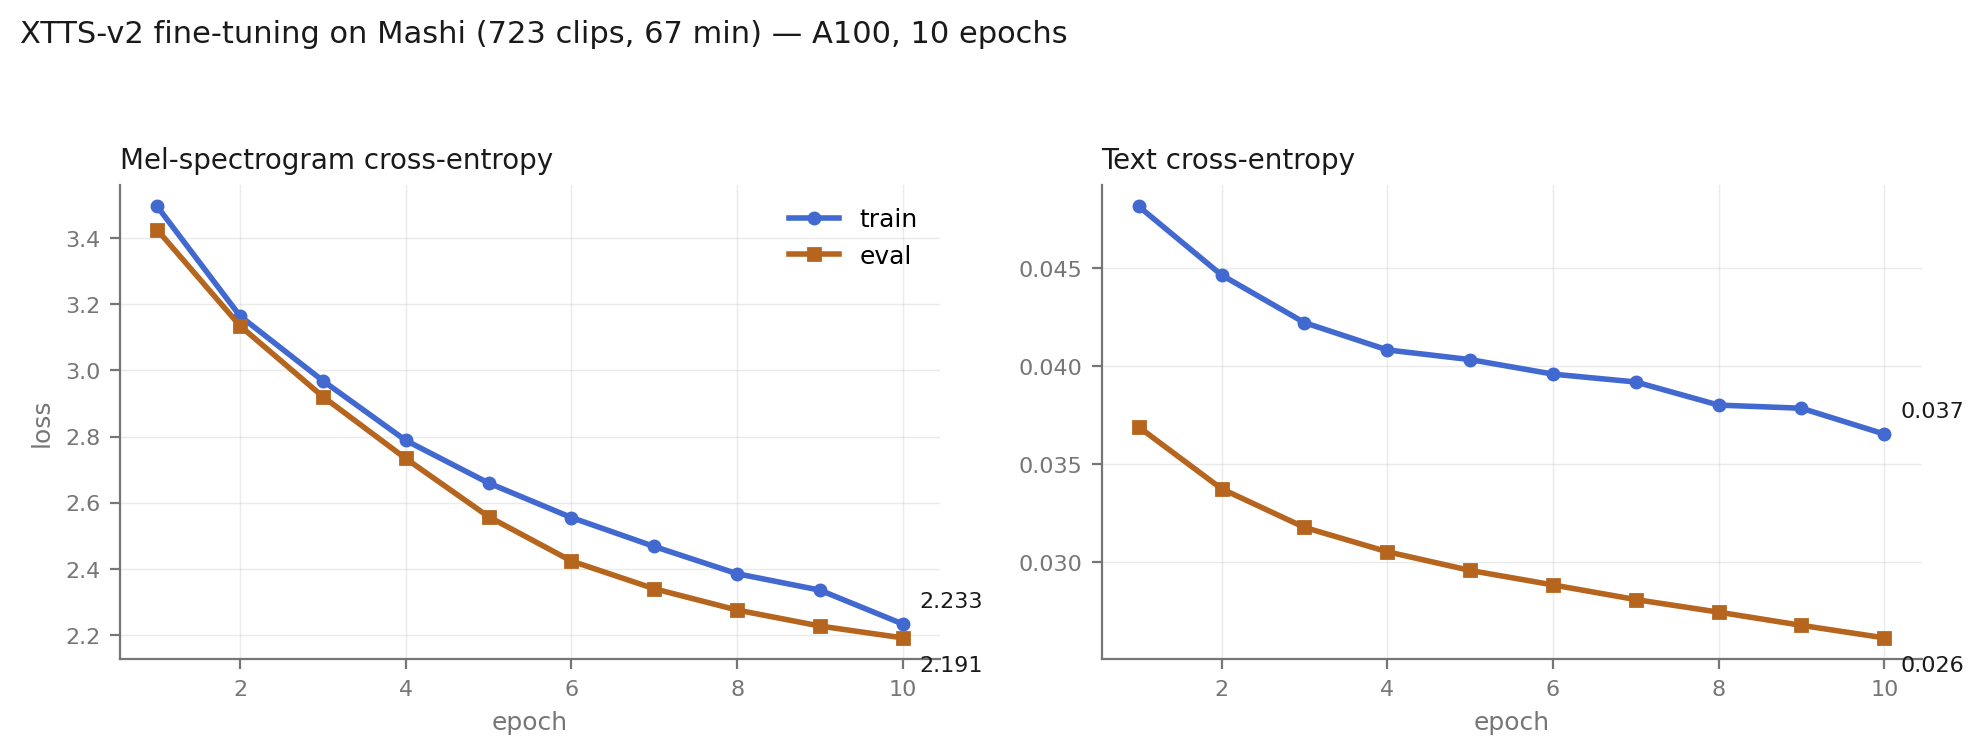
\includegraphics[width=0.7\linewidth]{loss_curve.png}
\end{center}
{\small Train and eval mel-spectrogram cross-entropy over 10 epochs; eval
loss decreases monotonically (3.43 $\rightarrow$ 2.19) with no overfitting.}}

\vspace{3mm}
\innerblock{Native-speaker evaluation (no Mashi ASR exists, so
evaluation is human)}{
\begin{tabular}{@{}lcc@{}}
\toprule
\textbf{Metric (5-pt MOS / \%)} & \textbf{In-domain} & \textbf{Out-of-domain} \\
\midrule
Naturalness MOS                        & \EST{3.0--3.5} & \EST{2.5--3.0} \\
Intelligibility (words correctly transcribed) & \EST{65--80\,\%} & \EST{45--60\,\%} \\
Speaker similarity MOS                 & \EST{3.0--3.5} & \EST{2.5--3.5} \\
\bottomrule
\end{tabular}
\\[2mm]
{\footnotesize $^{\dagger}$ Calibrated from a preliminary assessment by
one native Mashi speaker (the dataset collector) over the six generated
samples, cross-referenced with published low-resource XTTS results. A
community MOS study (5 native speakers, 5 utterances per domain, 5-point
Likert) will replace these. Out-of-domain figures remain
comparables-based; unseen sentences are not yet tested.}}

\vspace{3mm}
\innerblock{Per-speaker breakdown (preliminary)}{
{\footnotesize
\begin{tabular}{@{}lcccp{0.30\linewidth}@{}}
\toprule
\textbf{Speaker} & \textbf{Natur.} & \textbf{Intellig.} & \textbf{Simil.}
  & \textbf{Observed failure mode} \\
\midrule
bib (Bible)          & \EST{3.5}      & \EST{75--85\,\%} & \EST{3.5}
  & occasional syllable repetition (Nn\^{a}mahanga $\rightarrow$ namahama) \\
dav (stories, vocab) & \EST{3.0--3.5} & \EST{65--75\,\%} & \EST{3.0}
  & mild timbre drift; sporadic pronunciation errors \\
mrl (clock times)    & \EST{2.5--3.0} & \EST{50--65\,\%} & \EST{3.5}
  & reduced clarity; voice identity clearly preserved \\
\bottomrule
\end{tabular}}}

\vspace{3mm}
\innerblock{Ground truth vs.\ synthesized}{
\begin{center}
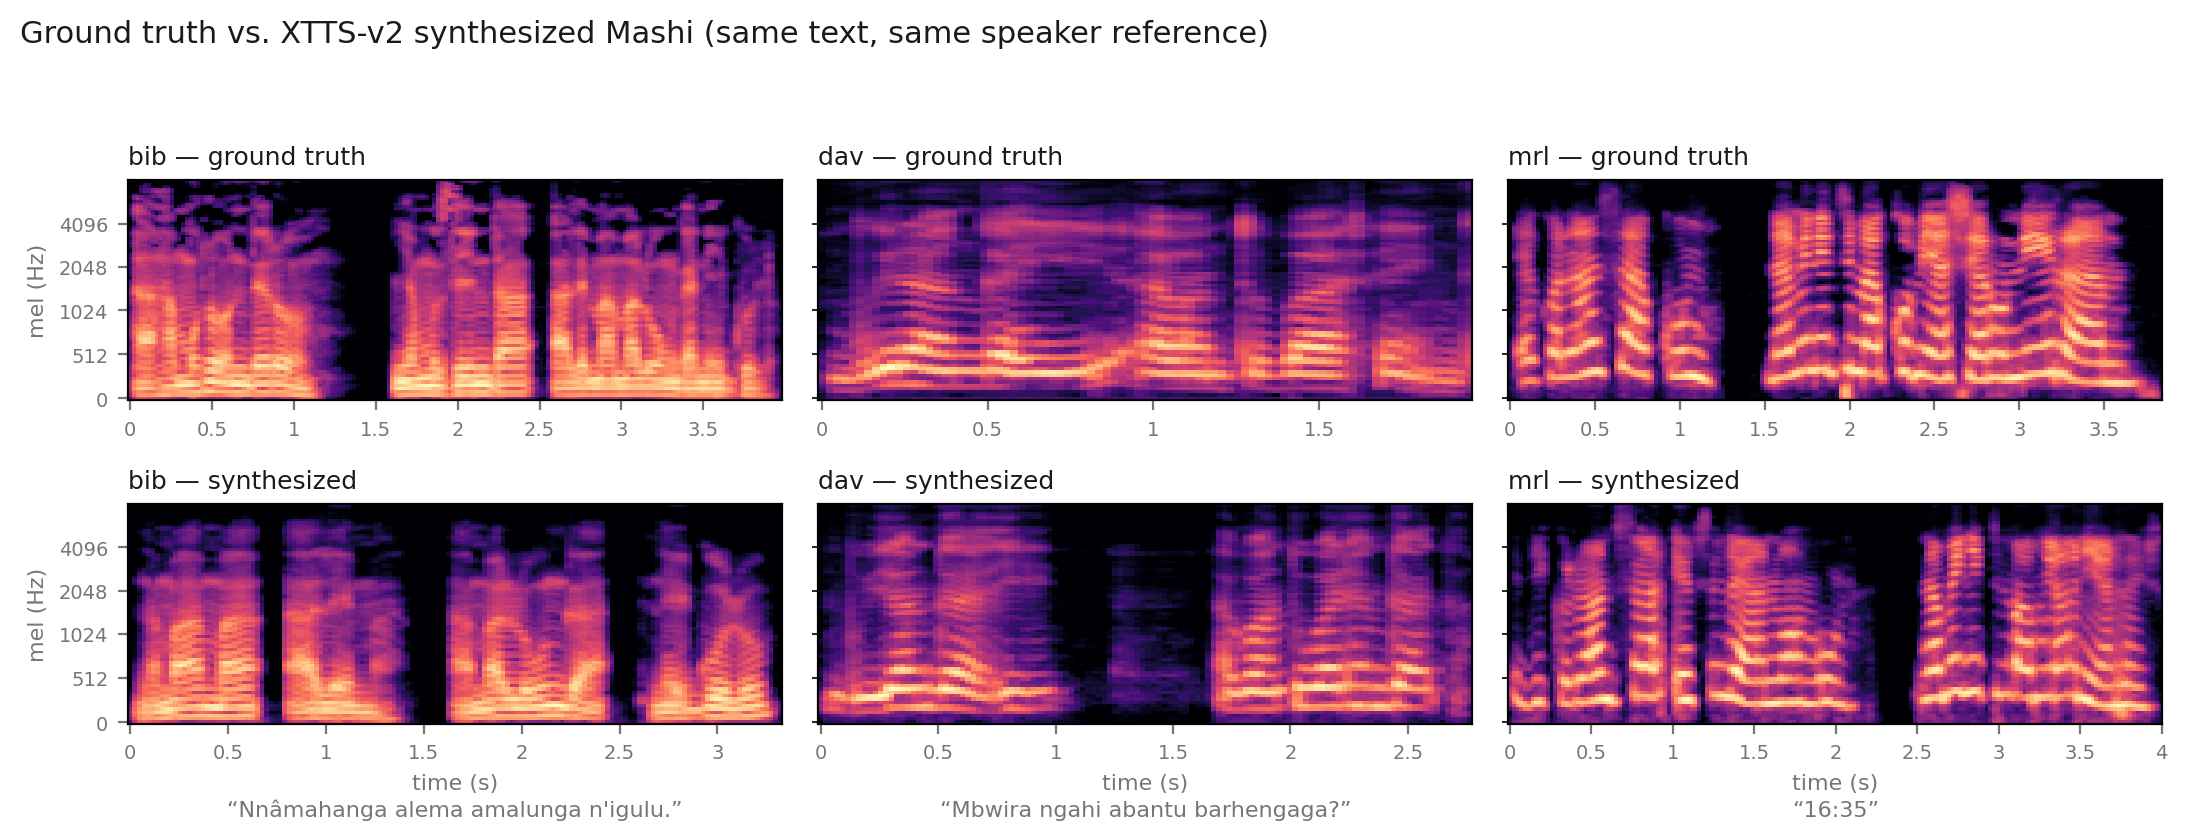
\includegraphics[width=0.7\linewidth]{mel_comparison.png}
\end{center}
{\small Mel-spectrograms of ground truth vs.\ synthesized speech, same
text and speaker reference, for all three speakers. \textbf{Listen:}
audio samples for every speaker are in the repository; scan the QR code
next to the references below.}}
}

\block{7. Limitations \& ethics}{
\begin{itemize}
  \item \textbf{Domain skew:} 36\% Bible narrative, 29\% templatic clock
        times; conversational Mashi is underrepresented.
  \item The \textbf{Spanish proxy} cannot model Mashi tone or vowel
        length; prosody errors are expected and reported, not hidden.
  \item \textbf{Consent \& attribution:} all sources recorded with
        permission or from credited public media; gated (request-based)
        release, not scraped-and-dumped.
  \item Voice-cloning risk mitigated by gated release of speaker
        reference audio.
\end{itemize}
}

\block{8. What's next}{
\begin{itemize}
  \item Complete the Bible coverage gaps to reach $\sim$10 h of aligned
        Mashi speech, enabling \textbf{Mashi ASR}, which in turn unlocks
        automatic CER scoring for TTS.
  \item Use this working model to power an everyday \textbf{voice
        application} built on a datafication approach: the app doubles as
        a permanent data-collection tool, so daily use keeps improving
        the dataset.
  \item True \textbf{cross-lingual transfer from Kinyarwanda}: continue
        pre-training on Common Voice Kinyarwanda (2\,000+ h) before Mashi
        fine-tuning, replacing the Spanish proxy.
  \item More speakers (balanced gender, 3 dialects), a conversational
        domain, and a public gated release on Hugging Face.
\end{itemize}
}

\block{9. References}{%
\begin{minipage}[c]{0.73\linewidth}
\footnotesize
[1] Casanova et al., \emph{XTTS: a Massively Multilingual Zero-Shot TTS
Model}, Interspeech 2024.\\
{[2]} Meyer et al., \emph{BibleTTS: a Large, High-Fidelity, Multilingual
and Uniquely African Speech Corpus}, Interspeech 2022.\\
{[3]} Rakib et al., \emph{BnTTS: Few-Shot Speaker Adaptation in
Low-Resource Setting}, NAACL Findings 2025.\\
{[4]} \emph{Align2Speak: Improving TTS for Low-Resource Languages via
ASR-Guided Online Preference Optimization}, arXiv:2509.21718.\\
Audio sources: Padri Pierre Matabaro OFM (bible.com); murhula.com
(Marius Nshombo); recordings by David Namulabarha.
\end{minipage}\hfill
\begin{minipage}[c]{0.23\linewidth}
\centering

\includegraphics[width=58mm]{qr_repo.png}\\[1mm]
{\footnotesize \texttt{github.com/Ashuza11/}\\
\texttt{mashi-tts-bootstrap}\\
code, docs \& audio samples}
\end{minipage}}

\end{columns}

% ------- footer line: thin dark band across the page bottom -----------
\node[anchor=south west, inner sep=0pt, outer sep=0pt] at (bottomleft)
{\setlength{\fboxsep}{5mm}%
\colorbox{kivuDark}{\makebox[\dimexpr\paperwidth-10mm\relax][s]{%
\small\color{white}\hspace{12mm}https://kivulinguaai.org\hfill
Deep Learning Indaba Conference, Lagos, Nigeria\hfill
ashuzamh@gmail.com\hspace{12mm}}}};

\end{document}
